\section{Overview of the build data}

\begin{figure*}[!h]
\subfloat[]{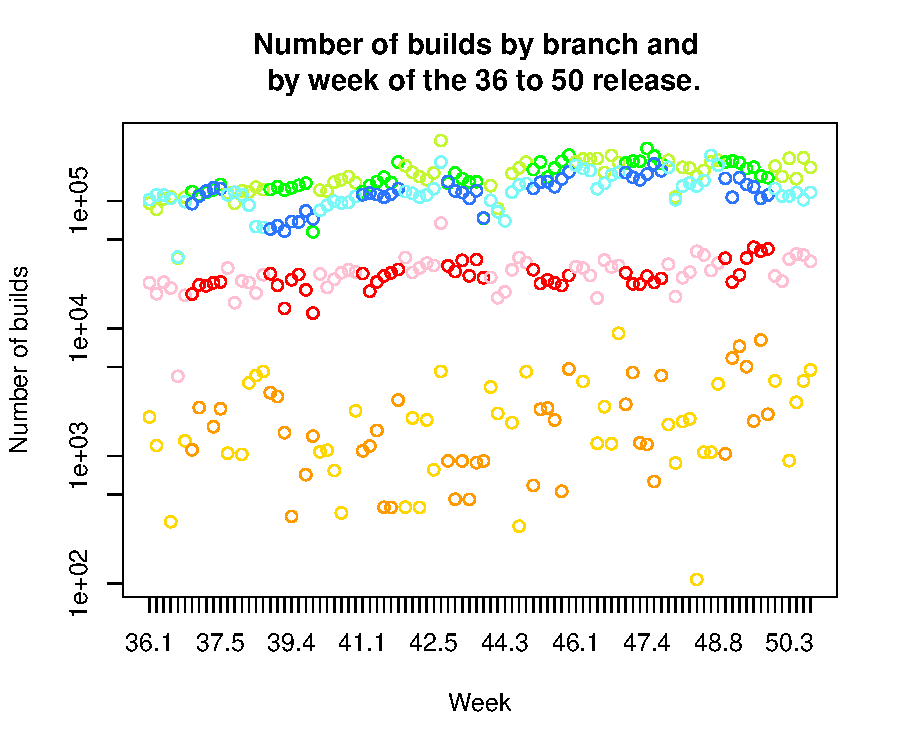
\includegraphics[clip, width=0.3\textwidth]{img/build_week.pdf}}
\hfill
\subfloat[]{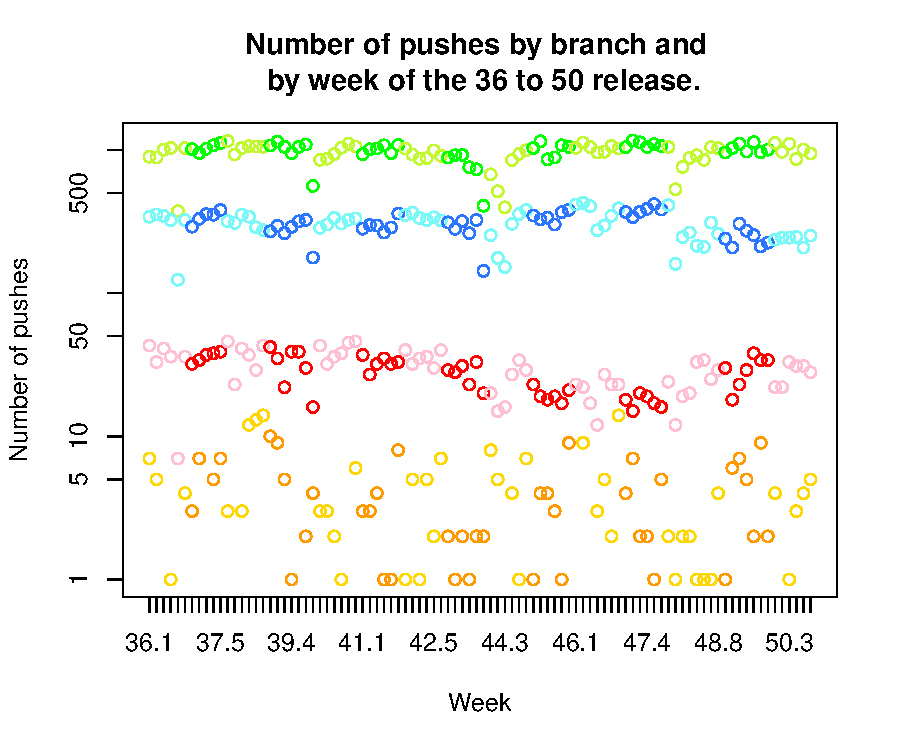
\includegraphics[clip, width=0.3\textwidth]{img/push_week.pdf}}
\hfill
\subfloat[]{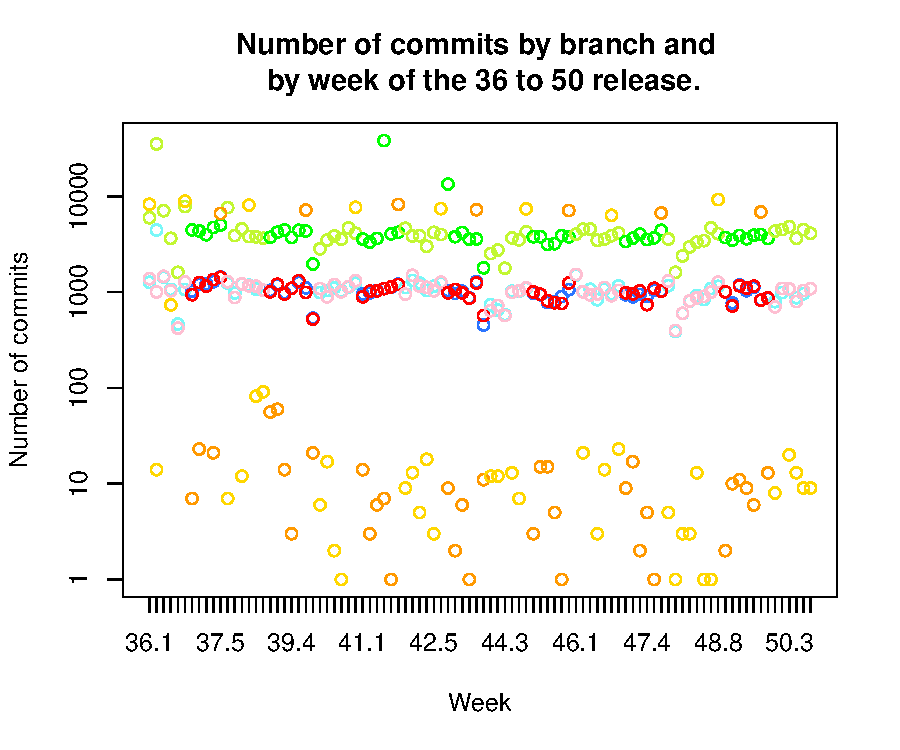
\includegraphics[clip, width=0.3\textwidth]{img/commit_week.pdf}}\\
\caption{\label{byweek}Quantitative values by week computed on the build dataset. (a) Number of builds by week. (b) Number of pushes by week. (c) Number of commits by week. }
\end{figure*}



%\kyle{The higher number of pushes from release 36 to 44 on the mozilla-central branch on Fig~\ref{byweek}(a) would reduce and be more stable over time if we would ignore the pushes not found on mercurial (43\% of the pushes of that branch, see the first two pages of the report). For the rest, does those results seems logical to you regarding the purpose of each branch ?}

\kyle{Do those results seem logical to you regarding the purpose of each branch ? }
\newpage